% ============================================================
% Question Bank: ch01-01 Unit Rates with Fractions
% Topic Title: Unit Rates with Fractions
% CCSS: 7.RP.A.1
% Questions: 27 (15 MC + 6 SA + 6 Graphical)
% ============================================================

% --- Multiple Choice Questions (15) ---

\begin{practiceQuestion}{1-1-q01}{mc}
\begin{questionText}
A gardener uses $\frac{2}{5}$ bag of soil to fill $\frac{1}{3}$ of a planter box. How many bags of soil are needed to fill the entire planter box?
\end{questionText}
\choiceA{$\frac{2}{15}$}
\choiceB{$\frac{6}{5}$}
\choiceC{$1\frac{1}{5}$}
\choiceD{$1\frac{2}{5}$}
\correctAnswer{C}
\explanation{To find the unit rate, divide bags by the fraction filled: $\frac{2}{5} \div \frac{1}{3} = \frac{2}{5} \times \frac{3}{1} = \frac{6}{5} = 1\frac{1}{5}$ bags per planter box.}
\end{practiceQuestion}

\begin{practiceQuestion}{1-1-q02}{mc}
\begin{questionText}
A cyclist rides $\frac{3}{4}$ mile in $\frac{2}{5}$ hour. What is the cyclist's speed in miles per hour?
\end{questionText}
\choiceA{$\frac{3}{10}$ mph}
\choiceB{$\frac{8}{15}$ mph}
\choiceC{$1\frac{7}{8}$ mph}
\choiceD{$1\frac{1}{4}$ mph}
\correctAnswer{C}
\explanation{Divide the distance by the time to find the unit rate: $\frac{3}{4} \div \frac{2}{5} = \frac{3}{4} \times \frac{5}{2} = \frac{15}{8} = 1\frac{7}{8}$ miles per hour.}
\end{practiceQuestion}

\begin{practiceQuestion}{1-1-q03}{mc}
\begin{questionText}
A bakery uses $\frac{7}{8}$ pound of butter in $\frac{1}{4}$ hour. At this rate, how many pounds of butter does the bakery use per hour?
\end{questionText}
\choiceA{$\frac{7}{32}$ lb}
\choiceB{$2\frac{1}{2}$ lb}
\choiceC{$3$ lb}
\choiceD{$3\frac{1}{2}$ lb}
\correctAnswer{D}
\explanation{Divide pounds by hours: $\frac{7}{8} \div \frac{1}{4} = \frac{7}{8} \times \frac{4}{1} = \frac{28}{8} = \frac{7}{2} = 3\frac{1}{2}$ pounds per hour.}
\end{practiceQuestion}

\begin{practiceQuestion}{1-1-q04}{mc}
\begin{questionText}
A volunteer paints $\frac{2}{5}$ of a mural in $\frac{3}{4}$ hour. At this rate, what fraction of the mural can the volunteer paint in one hour?
\end{questionText}
\choiceA{$\frac{3}{10}$}
\choiceB{$\frac{8}{15}$}
\choiceC{$\frac{3}{5}$}
\choiceD{$\frac{6}{20}$}
\correctAnswer{B}
\explanation{Divide the fraction of the mural by the time: $\frac{2}{5} \div \frac{3}{4} = \frac{2}{5} \times \frac{4}{3} = \frac{8}{15}$ of the mural per hour.}
\end{practiceQuestion}

\begin{practiceQuestion}{1-1-q05}{mc}
\begin{questionText}
A factory assembles $\frac{5}{6}$ of a product in $\frac{5}{12}$ hour. How many complete products does the factory assemble per hour?
\end{questionText}
\choiceA{$\frac{25}{72}$}
\choiceB{$1$}
\choiceC{$2$}
\choiceD{$2\frac{1}{2}$}
\correctAnswer{C}
\explanation{Divide products by hours: $\frac{5}{6} \div \frac{5}{12} = \frac{5}{6} \times \frac{12}{5} = \frac{60}{30} = 2$ products per hour.}
\end{practiceQuestion}

\begin{practiceQuestion}{1-1-q06}{mc}
\begin{questionText}
A water pipe fills $\frac{2}{3}$ of a pool in $\frac{5}{6}$ hour. Which expression correctly shows how to find the filling rate in pools per hour?
\end{questionText}
\choiceA{$\frac{2}{3} \times \frac{5}{6}$}
\choiceB{$\frac{5}{6} \div \frac{2}{3}$}
\choiceC{$\frac{2}{3} \div \frac{5}{6}$}
\choiceD{$\frac{2}{3} + \frac{5}{6}$}
\correctAnswer{C}
\explanation{A unit rate is found by dividing the first quantity by the second: pools $\div$ hours $= \frac{2}{3} \div \frac{5}{6}$. This gives $\frac{2}{3} \times \frac{6}{5} = \frac{4}{5}$ pool per hour.}
\end{practiceQuestion}

\begin{practiceQuestion}{1-1-q07}{mc}
\begin{questionText}
Jasmine jogs $\frac{4}{5}$ mile in $\frac{1}{3}$ hour. Marcus jogs $\frac{5}{6}$ mile in $\frac{1}{2}$ hour. Who jogs at a faster rate?
\end{questionText}
\choiceA{Jasmine, at $2\frac{2}{5}$ mph}
\choiceB{Marcus, at $1\frac{2}{3}$ mph}
\choiceC{They jog at the same rate}
\choiceD{Jasmine, at $2\frac{2}{3}$ mph}
\correctAnswer{A}
\explanation{Find each unit rate. Jasmine: $\frac{4}{5} \div \frac{1}{3} = \frac{4}{5} \times 3 = \frac{12}{5} = 2\frac{2}{5}$ mph. Marcus: $\frac{5}{6} \div \frac{1}{2} = \frac{5}{6} \times 2 = \frac{10}{6} = 1\frac{2}{3}$ mph. Since $2\frac{2}{5} > 1\frac{2}{3}$, Jasmine is faster.}
\end{practiceQuestion}

\begin{practiceQuestion}{1-1-q08}{mc}
\begin{questionText}
A truck delivers $\frac{3}{4}$ ton of gravel in $\frac{2}{3}$ trip. How many tons of gravel are delivered per trip?
\end{questionText}
\choiceA{$\frac{1}{2}$ ton}
\choiceB{$\frac{9}{8}$ tons}
\choiceC{$1\frac{1}{8}$ tons}
\choiceD{$1\frac{1}{2}$ tons}
\correctAnswer{C}
\explanation{Divide tons by trips: $\frac{3}{4} \div \frac{2}{3} = \frac{3}{4} \times \frac{3}{2} = \frac{9}{8} = 1\frac{1}{8}$ tons per trip. Note that choices B and C show the same value in different forms; $\frac{9}{8} = 1\frac{1}{8}$.}
\end{practiceQuestion}

\begin{practiceQuestion}{1-1-q09}{mc}
\begin{questionText}
A student says the unit rate for $\frac{1}{2}$ gallon in $\frac{3}{4}$ minute is $\frac{3}{8}$ gallon per minute. Which best describes the student's error?
\end{questionText}
\choiceA{The student multiplied instead of dividing.}
\choiceB{The student found the reciprocal of the wrong fraction.}
\choiceC{The student forgot to simplify the answer.}
\choiceD{The student switched the numerator and denominator of the answer.}
\correctAnswer{A}
\explanation{The student multiplied $\frac{1}{2} \times \frac{3}{4} = \frac{3}{8}$ instead of dividing. The correct computation is $\frac{1}{2} \div \frac{3}{4} = \frac{1}{2} \times \frac{4}{3} = \frac{2}{3}$ gallon per minute.}
\end{practiceQuestion}

\begin{practiceQuestion}{1-1-q10}{mc}
\begin{questionText}
A lawnmower uses $\frac{1}{3}$ gallon of gas to mow $\frac{5}{8}$ of a yard. How much gas is needed to mow one full yard?
\end{questionText}
\choiceA{$\frac{5}{24}$ gallon}
\choiceB{$\frac{8}{15}$ gallon}
\choiceC{$\frac{15}{8}$ gallons}
\choiceD{$1\frac{7}{8}$ gallons}
\correctAnswer{B}
\explanation{Divide gas by fraction of yard: $\frac{1}{3} \div \frac{5}{8} = \frac{1}{3} \times \frac{8}{5} = \frac{8}{15}$ gallon per yard.}
\end{practiceQuestion}

\begin{practiceQuestion}{1-1-q11}{mc}
\begin{questionText}
Ribbon A costs $\frac{3}{5}$ dollar per $\frac{1}{2}$ yard. Ribbon B costs $\frac{4}{7}$ dollar per $\frac{1}{3}$ yard. Which ribbon has the lower price per yard?
\end{questionText}
\choiceA{Ribbon A at $\$1\frac{1}{5}$ per yard}
\choiceB{Ribbon B at $\$1\frac{5}{7}$ per yard}
\choiceC{Ribbon A at $\$\frac{3}{10}$ per yard}
\choiceD{They have the same price per yard}
\correctAnswer{A}
\explanation{Find each unit rate. Ribbon A: $\frac{3}{5} \div \frac{1}{2} = \frac{3}{5} \times 2 = \frac{6}{5} = 1\frac{1}{5}$ dollars per yard. Ribbon B: $\frac{4}{7} \div \frac{1}{3} = \frac{4}{7} \times 3 = \frac{12}{7} = 1\frac{5}{7}$ dollars per yard. Ribbon A is cheaper.}
\end{practiceQuestion}

\begin{practiceQuestion}{1-1-q12}{mc}
\begin{questionText}
A printer uses $\frac{2}{3}$ of an ink cartridge to print $\frac{4}{5}$ of a manual. At this rate, how many ink cartridges are needed to print the full manual?
\end{questionText}
\choiceA{$\frac{8}{15}$}
\choiceB{$\frac{5}{6}$}
\choiceC{$1\frac{1}{6}$}
\choiceD{$1\frac{7}{12}$}
\correctAnswer{B}
\explanation{Divide cartridges by fraction of the manual: $\frac{2}{3} \div \frac{4}{5} = \frac{2}{3} \times \frac{5}{4} = \frac{10}{12} = \frac{5}{6}$ cartridge per full manual.}
\end{practiceQuestion}

\begin{practiceQuestion}{1-1-q13}{mc}
\begin{questionText}
An artist mixes $\frac{3}{8}$ ounce of blue paint with $\frac{1}{6}$ ounce of white paint per batch. What is the unit rate of blue paint to white paint in ounces of blue per ounce of white?
\end{questionText}
\choiceA{$\frac{1}{16}$}
\choiceB{$\frac{4}{9}$}
\choiceC{$2\frac{1}{4}$}
\choiceD{$2\frac{1}{2}$}
\correctAnswer{C}
\explanation{Divide blue by white: $\frac{3}{8} \div \frac{1}{6} = \frac{3}{8} \times \frac{6}{1} = \frac{18}{8} = \frac{9}{4} = 2\frac{1}{4}$ ounces of blue per ounce of white.}
\end{practiceQuestion}

\begin{practiceQuestion}{1-1-q14}{mc}
\begin{questionText}
A worker digs $\frac{1}{4}$ of a trench in $\frac{2}{5}$ hour. Another worker digs $\frac{1}{3}$ of the same trench in $\frac{1}{2}$ hour. Which worker digs at a faster rate?
\end{questionText}
\choiceA{First worker at $\frac{5}{8}$ trench per hour}
\choiceB{Second worker at $\frac{2}{3}$ trench per hour}
\choiceC{First worker at $\frac{2}{5}$ trench per hour}
\choiceD{They dig at the same rate}
\correctAnswer{B}
\explanation{First worker: $\frac{1}{4} \div \frac{2}{5} = \frac{1}{4} \times \frac{5}{2} = \frac{5}{8}$ trench per hour. Second worker: $\frac{1}{3} \div \frac{1}{2} = \frac{1}{3} \times 2 = \frac{2}{3}$ trench per hour. Since $\frac{2}{3} > \frac{5}{8}$, the second worker is faster.}
\end{practiceQuestion}

\begin{practiceQuestion}{1-1-q15}{mc}
\begin{questionText}
A recipe calls for $\frac{5}{6}$ cup of milk to make $\frac{2}{3}$ of a batch of pancakes. Elena says each full batch needs $1\frac{1}{4}$ cups of milk. Is Elena correct?
\end{questionText}
\choiceA{Yes, because $\frac{5}{6} \div \frac{2}{3} = 1\frac{1}{4}$}
\choiceB{No, the answer is $\frac{5}{9}$ cup}
\choiceC{No, the answer is $1\frac{1}{2}$ cups}
\choiceD{Yes, because $\frac{5}{6} \times \frac{2}{3} = 1\frac{1}{4}$}
\correctAnswer{A}
\explanation{Divide cups by fraction of batch: $\frac{5}{6} \div \frac{2}{3} = \frac{5}{6} \times \frac{3}{2} = \frac{15}{12} = \frac{5}{4} = 1\frac{1}{4}$. Elena is correct.}
\end{practiceQuestion}

% --- Short Answer Questions (6) ---

\begin{practiceQuestion}{1-1-q16}{sa}
\begin{questionText}
A sprinkler waters $\frac{3}{5}$ of a garden in $\frac{1}{2}$ hour. At this rate, what fraction of the garden does the sprinkler water per hour?
\end{questionText}
\correctAnswer{$1\frac{1}{5}$}
\explanation{Divide the fraction of the garden by the time: $\frac{3}{5} \div \frac{1}{2} = \frac{3}{5} \times 2 = \frac{6}{5} = 1\frac{1}{5}$ gardens per hour.}
\end{practiceQuestion}

\begin{practiceQuestion}{1-1-q17}{sa}
\begin{questionText}
A carpenter sands $\frac{5}{8}$ of a tabletop in $\frac{3}{4}$ hour. What is the unit rate in tabletops per hour?
\end{questionText}
\correctAnswer{$\frac{5}{6}$}
\explanation{Divide tabletop fraction by hours: $\frac{5}{8} \div \frac{3}{4} = \frac{5}{8} \times \frac{4}{3} = \frac{20}{24} = \frac{5}{6}$ tabletop per hour.}
\end{practiceQuestion}

\begin{practiceQuestion}{1-1-q18}{sa}
\begin{questionText}
Tomato sauce A uses $\frac{1}{4}$ cup of olive oil for $\frac{2}{3}$ cup of tomatoes. How many cups of olive oil are used per cup of tomatoes?
\end{questionText}
\correctAnswer{$\frac{3}{8}$}
\explanation{Divide olive oil by tomatoes: $\frac{1}{4} \div \frac{2}{3} = \frac{1}{4} \times \frac{3}{2} = \frac{3}{8}$ cup of olive oil per cup of tomatoes.}
\end{practiceQuestion}

\begin{practiceQuestion}{1-1-q19}{sa}
\begin{questionText}
A train covers $\frac{7}{10}$ mile in $\frac{2}{5}$ minute. What is the train's speed in miles per minute?
\end{questionText}
\correctAnswer{$1\frac{3}{4}$}
\explanation{Divide distance by time: $\frac{7}{10} \div \frac{2}{5} = \frac{7}{10} \times \frac{5}{2} = \frac{35}{20} = \frac{7}{4} = 1\frac{3}{4}$ miles per minute.}
\end{practiceQuestion}

\begin{practiceQuestion}{1-1-q20}{sa}
\begin{questionText}
A smoothie recipe uses $\frac{2}{3}$ cup of yogurt and $\frac{3}{4}$ cup of fruit. What is the unit rate of yogurt to fruit in cups of yogurt per cup of fruit?
\end{questionText}
\correctAnswer{$\frac{8}{9}$}
\explanation{Divide yogurt by fruit: $\frac{2}{3} \div \frac{3}{4} = \frac{2}{3} \times \frac{4}{3} = \frac{8}{9}$ cup of yogurt per cup of fruit.}
\end{practiceQuestion}

\begin{practiceQuestion}{1-1-q21}{sa}
\begin{questionText}
DeShaun reads $\frac{3}{7}$ of a chapter in $\frac{1}{3}$ hour. Priya reads $\frac{2}{5}$ of the same chapter in $\frac{1}{4}$ hour. How much faster is the faster reader, in chapters per hour?
\end{questionText}
\correctAnswer{$\frac{11}{35}$}
\explanation{DeShaun: $\frac{3}{7} \div \frac{1}{3} = \frac{9}{7}$ chapters per hour. Priya: $\frac{2}{5} \div \frac{1}{4} = \frac{8}{5}$ chapters per hour. Difference: $\frac{8}{5} - \frac{9}{7} = \frac{56}{35} - \frac{45}{35} = \frac{11}{35}$ chapter per hour faster.}
\end{practiceQuestion}

% --- Graphical Multiple Choice Questions (3) ---

\begin{practiceQuestion}{1-1-q22}{gmc}
\begin{questionText}
The table below shows the amount of fabric used and the number of scarves made at a costume shop.

\begin{center}
\begin{tabular}{|c|c|}
\hline
\textbf{Scarves} & \textbf{Fabric (yards)} \\
\hline
$\frac{1}{4}$ & $\frac{3}{8}$ \\[4pt]
$\frac{1}{2}$ & $\frac{3}{4}$ \\[4pt]
$1$ & $?$ \\
\hline
\end{tabular}
\end{center}

What is the unit rate of fabric per scarf?
\end{questionText}
\choiceA{$\frac{3}{32}$ yard per scarf}
\choiceB{$\frac{2}{3}$ yard per scarf}
\choiceC{$1\frac{1}{2}$ yards per scarf}
\choiceD{$3$ yards per scarf}
\correctAnswer{C}
\explanation{Divide fabric by scarves using the first row: $\frac{3}{8} \div \frac{1}{4} = \frac{3}{8} \times 4 = \frac{12}{8} = \frac{3}{2} = 1\frac{1}{2}$ yards per scarf.}
\end{practiceQuestion}

\begin{practiceQuestion}{1-1-q23}{gmc}
\begin{questionText}
The bar graph below shows the distance two runners covered in $\frac{1}{3}$ hour.

\begin{center}
\begin{tikzpicture}[scale=0.8]
  \draw[thick,->] (0,0) -- (0,4.5) node[above]{\small Miles};
  \draw[thick,->] (0,0) -- (5,0);
  \fill[funBlue] (0.5,0) rectangle (2,3);
  \fill[funOrange] (2.5,0) rectangle (4,2.5);
  \node[below] at (1.25,0) {\small Runner A};
  \node[below] at (3.25,0) {\small Runner B};
  \foreach \y/\lab in {1/\frac{1}{4},2/\frac{1}{2},3/\frac{3}{4},4/1}
    \draw (-0.1,\y) -- (0.1,\y) node[left=4pt] {$\lab$};
\end{tikzpicture}
\end{center}

Which runner has the faster speed in miles per hour?
\end{questionText}
\choiceA{Runner A at $2\frac{1}{4}$ mph}
\choiceB{Runner B at $1\frac{7}{8}$ mph}
\choiceC{Runner A at $\frac{1}{4}$ mph}
\choiceD{Runner B at $1\frac{1}{2}$ mph}
\correctAnswer{A}
\explanation{From the graph, Runner A covers $\frac{3}{4}$ mile and Runner B covers about $\frac{5}{8}$ mile in $\frac{1}{3}$ hour. Runner A: $\frac{3}{4} \div \frac{1}{3} = \frac{3}{4} \times 3 = \frac{9}{4} = 2\frac{1}{4}$ mph. Runner B: $\frac{5}{8} \div \frac{1}{3} = \frac{5}{8} \times 3 = \frac{15}{8} = 1\frac{7}{8}$ mph. Runner A is faster.}
\end{practiceQuestion}

\begin{practiceQuestion}{1-1-q24}{gmc}
\begin{questionText}
The number line below is labeled in fourths. A snail moves from $0$ to point $P$ in $\frac{2}{3}$ hour.

\begin{center}
\begin{tikzpicture}
  \draw[thick,->] (-0.5,0) -- (5.5,0);
  \foreach \x/\lab in {0/0,1/\frac{1}{4},2/\frac{1}{2},3/\frac{3}{4},4/1,5/1\frac{1}{4}}
    \draw (\x,0.15) -- (\x,-0.15) node[below]{$\lab$};
  \fill[funRed] (3,0) circle (4pt) node[above=4pt]{\small $P$};
\end{tikzpicture}
\end{center}

What is the snail's speed in units per hour?
\end{questionText}
\choiceA{$\frac{1}{2}$}
\choiceB{$\frac{3}{4}$}
\choiceC{$1\frac{1}{8}$}
\choiceD{$1\frac{1}{4}$}
\correctAnswer{C}
\explanation{Point $P$ is at $\frac{3}{4}$ on the number line. The snail's speed is $\frac{3}{4} \div \frac{2}{3} = \frac{3}{4} \times \frac{3}{2} = \frac{9}{8} = 1\frac{1}{8}$ units per hour.}
\end{practiceQuestion}

% --- Graphical Short Answer Questions (3) ---

\begin{practiceQuestion}{1-1-q25}{gsa}
\begin{questionText}
The table below shows the number of gallons of paint used and the area covered.

\begin{center}
\begin{tabular}{|c|c|}
\hline
\textbf{Paint (gallons)} & \textbf{Area (sq ft)} \\
\hline
$\frac{1}{3}$ & $100$ \\[4pt]
$\frac{2}{3}$ & $200$ \\[4pt]
$1$ & $?$ \\
\hline
\end{tabular}
\end{center}

How many square feet does one gallon of paint cover?
\end{questionText}
\correctAnswer{$300$}
\explanation{Divide area by paint: $100 \div \frac{1}{3} = 100 \times 3 = 300$ square feet per gallon. Check: $200 \div \frac{2}{3} = 200 \times \frac{3}{2} = 300$ \checkmark.}
\end{practiceQuestion}

\begin{practiceQuestion}{1-1-q26}{gsa}
\begin{questionText}
Two fraction bars are shown below, representing the distance two ants traveled in different times.

\begin{center}
Ant A: traveled \fractionBar[funBlue]{5}{8} mile in $\frac{1}{2}$ hour

\vspace{0.5em}
Ant B: traveled \fractionBar[funOrange]{3}{4} mile in $\frac{2}{3}$ hour
\end{center}

What is the difference between the two ants' speeds, in miles per hour?
\end{questionText}
\correctAnswer{$\frac{1}{8}$}
\explanation{Ant A: $\frac{5}{8} \div \frac{1}{2} = \frac{5}{8} \times 2 = \frac{10}{8} = \frac{5}{4} = 1\frac{1}{4}$ mph. Ant B: $\frac{3}{4} \div \frac{2}{3} = \frac{3}{4} \times \frac{3}{2} = \frac{9}{8} = 1\frac{1}{8}$ mph. Difference: $\frac{5}{4} - \frac{9}{8} = \frac{10}{8} - \frac{9}{8} = \frac{1}{8}$ mph.}
\end{practiceQuestion}

\begin{practiceQuestion}{1-1-q27}{gsa}
\begin{questionText}
The double number line below shows cups of sugar and batches of cookies.

\begin{center}
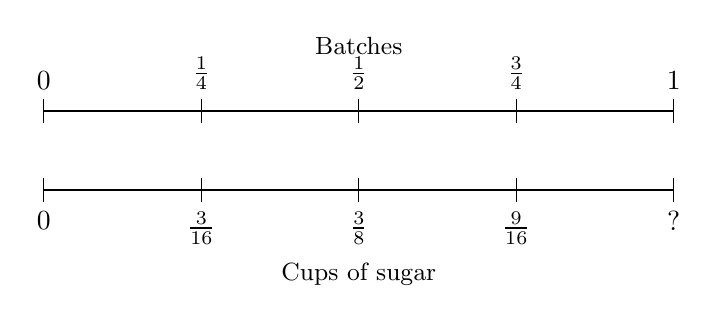
\begin{tikzpicture}[scale=1]
  \draw[thick] (0,0.5) -- (8,0.5);
  \draw[thick] (0,-0.5) -- (8,-0.5);
  \foreach \x/\lab in {0/0, 2/\frac{1}{4}, 4/\frac{1}{2}, 6/\frac{3}{4}, 8/1}
    \draw (\x,0.35) -- (\x,0.65) node[above]{$\lab$};
  \node[above] at (4,1.1) {\small Batches};
  \foreach \x/\lab in {0/0, 2/\frac{3}{16}, 4/\frac{3}{8}, 6/\frac{9}{16}, 8/?}
    \draw (\x,-0.35) -- (\x,-0.65) node[below]{$\lab$};
  \node[below] at (4,-1.3) {\small Cups of sugar};
\end{tikzpicture}
\end{center}

How many cups of sugar are needed for $1$ full batch of cookies?
\end{questionText}
\correctAnswer{$\frac{3}{4}$}
\explanation{From the double number line, $\frac{1}{4}$ batch uses $\frac{3}{16}$ cup. Find the unit rate: $\frac{3}{16} \div \frac{1}{4} = \frac{3}{16} \times 4 = \frac{12}{16} = \frac{3}{4}$ cup per batch.}
\end{practiceQuestion}
